% =========================================================================
% ICDEES 2026 Conference Paper Manuscript (IEEE Format)
% Venue: International Conference on Digital Economy and Emerging Societies (ICDEES 2026)
% IEEE Proceedings / IEEE Xplore Indexing
% Formatting: IEEEtran Conference (Double-Blind Review Ready)
% Structure: IMRaD (Introduction, Method, Result, Discussion, Conclusion)
% Target Length: Strictly 6 Pages Maximum (No Page 7 Spillover)
% =========================================================================

\documentclass[conference]{IEEEtran}
\IEEEoverridecommandlockouts

% -------------------------------------------------------------------------
% Core Packages & Typographical Optimization
% -------------------------------------------------------------------------
\usepackage{cite}
\usepackage{amsmath,amssymb,amsfonts}
\usepackage{algorithmic}
\usepackage{algorithm}
\usepackage{graphicx}
\usepackage{textcomp}
\usepackage{xcolor}
\usepackage{booktabs}
\usepackage{array}
\usepackage{adjustbox}
\usepackage{url}
\usepackage{hyperref}
\usepackage{microtype}

% -------------------------------------------------------------------------
% Float Spacing Adjustments (Guarantees Strict 6-Page Fit)
% -------------------------------------------------------------------------
\setlength{\textfloatsep}{4.5pt plus 1pt minus 1pt}
\setlength{\floatsep}{3.5pt plus 1pt minus 1pt}
\setlength{\intextsep}{3.5pt plus 1pt minus 1pt}
\setlength{\abovecaptionskip}{2pt plus 0.5pt minus 0.5pt}
\setlength{\belowcaptionskip}{1.5pt plus 0.5pt minus 0.5pt}

% -------------------------------------------------------------------------
% TikZ Graphics
% -------------------------------------------------------------------------
\usepackage{tikz}
\usetikzlibrary{shapes.geometric, arrows.meta, positioning, calc, fit}

% -------------------------------------------------------------------------
% Graphics Search Paths
% -------------------------------------------------------------------------
\graphicspath{{charts_ieee/}{./charts_ieee/}{charts/v03/}{./charts/v03/}{src/v3-run/}{../../src/v3-run/}}

% -------------------------------------------------------------------------
% Keyword Header Renaming (Replacing Index Terms with Keywords)
% -------------------------------------------------------------------------
\renewcommand\IEEEkeywordsname{Keywords}

\begin{document}

% -------------------------------------------------------------------------
% TITLE & ANONYMOUS AUTHOR BLOCK (DOUBLE-BLIND PEER REVIEW)
% -------------------------------------------------------------------------
\title{Unsupervised Dual-Path Consensus Machine Learning and Operational Policy Framework for Village Fund Expenditure Anomaly Detection}

\author{\IEEEauthorblockN{Anonymous Author(s)}
\IEEEauthorblockA{\textit{Double-Blind Peer Review}\\
Affiliation(s) and Identity Redacted in Compliance with ICDEES 2026 Guidelines\\
Location Marker: XXX}
}

\maketitle

% -------------------------------------------------------------------------
% ABSTRACT
% -------------------------------------------------------------------------
\begin{abstract}
Indonesia transfers roughly Rp 71 trillion annually to 75,259 rural jurisdictions through its \textit{Dana Desa} (Village Fund) program. Conventional anti-corruption oversight relies on reactive judicial prosecutions that lag two to five years behind disbursement cycles. Supervised machine learning cannot fix this gap because operational administrative ledgers contain zero ground-truth fraud labels when funds are disbursed. Grounded in Design Science Research (DSR), Agency Theory, and the Fraud Diamond, this study develops and evaluates an unsupervised Dual-Path Consensus framework (\textbf{Protocol 2}) combining Isolation Forest (IF), Local Outlier Factor (LOF), and an 8-layer Reconstruction Dense Autoencoder (RDA) with an Operational Policy Mapping Layer across 96,778 transaction records (1,363 villages, 2023--2025) in Jambi Province. Compared to standard majority voting (\textbf{Protocol 1}), \textbf{Protocol 2} decouples local density isolates from multi-model global convergence ($\text{IF} \cap \text{RDA}$). This expands anomaly recall from 3,107 (3.12\%) to \textbf{7,153 consensus anomalous records (7.39\%)}, isolating \textbf{Rp 642.85 billion in realization risk (14.89\%)} and \textbf{Rp 6.08 trillion in budget ceiling exposure (7.46\%)}. Operational policy mapping reveals a major typology shift toward \textbf{T2: Ghost Activities (58.1\% / 4,155 records)} and \textbf{T5: Procurement Irregularities (32.8\% / 2,343 records)}. Longitudinal tracking isolates \textbf{702 persistent Tier-1 villages (51.5\%)} flagged across all three fiscal years. On an ex-ante synthetic fraud benchmark ($N=10,000$, 5.0\% prevalence), \textbf{Protocol 2} achieves superior detection recovery (\textbf{Precision = 0.846, Recall = 0.846, F1 = 0.846, AUC-ROC = 0.912} vs. \textbf{Protocol 1} F1 = 0.568). Grounded in the DeLone \& McLean IS Success Model, the framework shrinks inspectorate audit search space by 92.6\% and translates neural reconstruction loss into actionable Explainable AI (XAI) field checklists.
\end{abstract}

\begin{IEEEkeywords}
Unsupervised Anomaly Detection, Dual-Path Consensus, Design Science Research, Reconstruction Autoencoder, Explainable AI, Village Fund Governance.
\end{IEEEkeywords}

% -------------------------------------------------------------------------
% SECTION I: INTRODUCTION
% -------------------------------------------------------------------------
\section{Introduction}

Indonesia transfers roughly Rp 71 trillion annually to 75,259 rural jurisdictions under Law No.\ 6 of 2014 on Villages~\cite{ref1}. But the sheer volume and speed of these disbursements outstrip local supervisory capacity. By 2024, Indonesia Corruption Watch (ICW) recorded 591 judicial convictions for village fund embezzlement, confirming Rp 598.13 billion in direct state losses~\cite{ref2}. Between 2015 and 2022 alone, the Corruption Eradication Commission (ACLC KPK) documented 851 corruption cases implicating 973 village apparatus members across Rp 468.9 trillion in disbursed funds~\cite{ref3}.

National anti-corruption agencies run several prevention initiatives: KPK's \textit{Trisula} strategy (Education, Prevention, Enforcement)~\cite{ref36}, the \textit{Desa Antikorupsi} pilot~\cite{ref37}, the BPKP-KPK \textit{Siswaskeudes} audit tool~\cite{ref38}, Stranas~PK 2025--2026 digital oversight~\cite{ref39}, the Monitoring Center for Prevention (MCP)~\cite{ref40}, and the \texttt{jaga.id} portal~\cite{ref26}. Yet these systems operate either at high municipal aggregates or rely on voluntary public whistleblower reports. None screens raw, activity-level transaction entries in \textit{Sistem Keuangan Desa} (Siskeudes) before annual disbursement tranches clear.

Prior research on rural fiscal oversight focuses heavily on qualitative administration~\cite{ref4,ref5} or classical fraud triangle diagnostics~\cite{ref6}. Where machine learning enters public sector auditing, researchers rely almost exclusively on supervised models~\cite{ref13,ref14}. That approach fails in practice: operational Siskeudes databases contain zero ground-truth fraud labels at the point of disbursement~\cite{ref16,ref23}. Auditors cannot train supervised classifiers on non-existent labels. We bridge this operational divide using Design Science Research (DSR)~\cite{ref5,ref10}. We build, evaluate, and compare an unsupervised Dual-Path Consensus artifact (\textbf{Protocol 2}) against a standard majority voting ensemble (\textbf{Protocol 1}) across 96,778 activity records from 1,363 villages in Jambi Province (FY 2023--2025).

\textbf{Jambi Province exposes this oversight deficit directly.} On KPK's \texttt{jaga.id} portal, Jambi registered just 11 citizen complaints (1.4\% of 761 national reports), despite having a comparable rural footprint to neighboring provinces~\cite{ref26}. As Alfada~\cite{ref27} demonstrates through panel GMM threshold modeling, heavy fiscal transfer dependency paired with weak citizen monitoring creates severe corruption exposure. Furthermore, district inspectorates (\textit{Aparat Pengawasan Intern Pemerintah} / APIP) employ only 5 to 15 field auditors per regency~\cite{ref12}, creating an impossible manual audit burden under Government Regulation No.\ 60/2008~\cite{ref33}. Recent prosecutions confirm that irregularities hide in plain sight within absorption ledgers: the \textit{Muara Hemat} case (Kerinci, Rp 644M loss, 5-year prosecution lag)~\cite{ref28,ref30}, the \textit{Jambi Tulo} freeze (Muaro Jambi, Rp 300M in fictitious projects)~\cite{ref29}, and the \textit{Pangkal Duri} trial (Tanjung Jabung Timur, Rp 415M loss)~\cite{ref31}. In each case, fictitious works, zero-realization procurement, and uncompetitive contracts sat unnoticed in administrative records for years.

This study delivers three core contributions:
\begin{enumerate}
    \item \textbf{Methodological Contribution}: We design an unsupervised Dual-Path Consensus framework combining local density estimation (LOF) and multi-model global convergence ($\text{IF} \cap \text{RDA}$) with an Operational Policy Mapping Layer, resolving the mutual cancellation failure of majority voting (\textbf{Protocol 1}).
    \item \textbf{Theoretical Contribution}: We operationalize Agency Theory, the Fraud Diamond, and Principal-Agent information asymmetry directly within administrative Siskeudes feature spaces.
    \item \textbf{Practical Contribution}: We deliver an operational screening framework that reduces APIP audit search space by 92.6\%, prioritizes 702 persistent Tier-1 villages, and translates neural autoencoder loss into Explainable AI (XAI) field checklists.
\end{enumerate}

This study answers three Research Questions (RQs):
\begin{itemize}
    \item \textbf{RQ1}: Which engineered feature constructs derived from Siskeudes records serve as the most discriminating signals of expenditure anomaly?
    \item \textbf{RQ2}: Which algorithmic ensemble architecture demonstrates superior anomaly discrimination on longitudinal village fund data?
    \item \textbf{RQ3}: How do algorithmically identified anomalies map to established corruption typologies, and how can XAI loss decomposition guide APIP field inspections?
\end{itemize}

% -------------------------------------------------------------------------
% SECTION II: METHODOLOGY & ARTIFACT ARCHITECTURE (IMRaD - Method)
% -------------------------------------------------------------------------
\section{Methodology \& Artifact Architecture}

\subsection{Theoretical Foundations \& Conceptual Framework}

Our artifact design builds on Agency Theory~\cite{ref25}, Wolfe \& Hermanson's Fraud Diamond~\cite{ref17b}, and the DeLone \& McLean IS Success Model~\cite{ref10}. Principal-Agent Theory frames the Village Head (\textit{Kepala Desa}) as an Agent holding private operational knowledge that the Principal (APIP inspectorates, BPKP, KPK) cannot directly observe:
\begin{equation}
\begin{aligned}
\mathrm{InfoAsymmetry} = {} & \mathcal{I}_{\mathrm{Agent}}(\mathrm{Realization}, \mathrm{TrueCost}) \\
& - \mathcal{I}_{\mathrm{Principal}}(\mathrm{SiskeudesReport})
\end{aligned}
\end{equation}
In Siskeudes execution, \textbf{Capability} sits with the Village Head and Financial Officer (\textit{Kaur Keuangan}), who manage digital credentials and banking authorization specimen signatures. \textbf{Opportunity} is built into procurement structures: \textbf{98.8\% of all village fund activities} in Jambi Province run through self-managed procurement (\textit{Swakelola}), bypassing competitive open market pricing~\cite{ref9}.

\begin{figure}[htbp]
\centering
\resizebox{\columnwidth}{!}{%
\begin{tikzpicture}[
    box/.style={draw=black!70, rectangle, rounded corners=3pt, align=center, minimum height=0.85cm, minimum width=2.0cm, fill=blue!5, font=\sffamily\scriptsize, line width=0.7pt},
    arrow/.style={-Stealth, thick, color=black!80, line width=0.9pt}
]
    \node[box, fill=red!10] (problem) {\textbf{Problem Domain}\\Rural Governance Deficit\\Siskeudes Signal Archive};
    \node[box, fill=amber!10, right=0.4cm of problem] (theory) {\textbf{Theory Foundation}\\Agency Asymmetry~\cite{ref25}\\Fraud Diamond~\cite{ref17b}};
    \node[box, fill=blue!10, right=0.4cm of theory] (artifact) {\textbf{DSR Artifact}\\Protocol 1: Majority\\Protocol 2: Dual-Path};
    \node[box, fill=green!10, right=0.4cm of artifact] (impact) {\textbf{IS Success Impact}\\92.6\% Search Reduction\\APIP Checklist~\cite{ref10}};

    \draw[arrow] (problem) -- (theory);
    \draw[arrow] (theory) -- (artifact);
    \draw[arrow] (artifact) -- (impact);
\end{tikzpicture}%
}
\caption{Integrated Conceptual Framework linking Agency Theory, Fraud Diamond, DSR Comparative Artifacts, and DeLone \& McLean IS Success Impact.}
\label{fig:conceptual_framework}
\end{figure}

\subsection{Data Hygiene \& Regional Baseline Centering}

The raw dataset (99,692 records) collected via KPK \texttt{jaga.id}~\cite{ref26} combines expenditure absorption (\textit{Penyerapan}) and budget ceiling (\textit{Pagu}) ledgers across FY 2023--2025. Data hygiene purges zero-volume entries and corrupt codes, leaving $N=96,778$ clean records across 1,363 villages.

To remove baseline price inflation caused by rugged highland geography and remote logistics costs (e.g., Kerinci highlands vs. Muaro Jambi lowlands), we compute year-stratified regional z-scores within each stratum $(c, k, t) = (\text{Kode\_Output}, \text{Kabupaten\_Kota}, \text{Tahun})$:
\begin{equation}
z_{i,c,k,t} = \frac{x_{i,c,k,t} - \mu_{c,k,t}}{\sigma_{c,k,t} + \epsilon}
\end{equation}
We then scale continuous features using \textbf{RobustScaler} (median centering, IQR scaling) to resist distortion from extreme price outliers. Table~\ref{tab:feature_matrix} details the 27-variable feature engineering matrix.

\begin{table}[htbp]
\centering
\caption{27-Variable Feature Engineering Matrix and Targeted Modus Operandi}
\label{tab:feature_matrix}
\setlength{\tabcolsep}{2.5pt}
\resizebox{\columnwidth}{!}{%
\begin{tabular}{lll}
\toprule
\textbf{Feature Construct} & \textbf{Mathematical Definition} & \textbf{Targeted Modus Operandi} \\
\midrule
\texttt{cost\_per\_unit} & $\text{Realization\_Total}_i / \text{Volume}_i$ (RobustScaler) & Unit price mark-up / inflation (T1) \\
\texttt{absorption\_ratio} & $\text{Realization\_Total}_i / \text{Pagu\_Village}_{v,t}$ & Ghost activity / zero progress (T2) \\
\texttt{avg\_completion} & $\frac{1}{3}(\text{Pct\_T1}_i + \text{Pct\_T2}_i + \text{Pct\_T3}_i)$ & Progress reporting manipulation \\
\texttt{swakelola\_high\_val} & $\mathbf{1}\left(\text{Swakelola}_i \land \text{Realization}_i > Q_{0.75}\right)$ & Uncompetitive procurement (T5) \\
\texttt{cost\_dev\_by\_cat} & $z_{i,c,k,t} = (x_{i,c,k,t} - \mu_{c,k,t}) / \sigma_{c,k,t}$ in $(c,k,t)$ & Regional price outlier (T7) \\
\texttt{n\_stages\_active} & $\sum_{m=1}^{3} \mathbf{1}\left(\text{Real\_T}m_i > 0\right)$ & Tranche draw concentration (T4) \\
\texttt{activity\_category} & One-Hot Encoded \texttt{Kode\_Output} (21 cats) & Cross-category dumping (T7) \\
\bottomrule
\end{tabular}%
}
\end{table}

\subsection{Multi-Paradigm Unsupervised Detection Engines}

The framework implements three orthogonal detection paradigms:

\subsubsection{1. Isolation Forest (Global Sparsity Engine)}
Isolation Forest partitions the feature space using recursive random splits~\cite{ref18}. Tree path length $h(x)$ across $T=200$ trees determines anomaly score $s(x, n) = 2^{-\mathbb{E}(h(x))/c(n)}$. Contamination $c = 0.10$ flags the top 10\% extreme global outliers:
\begin{equation}
y_{i, \mathrm{IF}} = \mathbf{1}\left(s(x_i, n) \ge \mathrm{Quantile}_{0.90}(s)\right)
\end{equation}

\subsubsection{2. Local Outlier Factor (Density Ratio Engine)}
LOF computes the local reachability density ($\text{lrd}_k$) ratio between instance $p$ and its $k=20$ nearest neighbors~\cite{ref24}:
\begin{equation}
\mathrm{LOF}_k(p) = \frac{1}{|N_k(p)|} \sum_{o \in N_k(p)} \frac{\mathrm{lrd}_k(o)}{\mathrm{lrd}_k(p)}
\end{equation}
\begin{equation}
y_{i, \mathrm{LOF}} = \mathbf{1}\left(\mathrm{LOF}_k(x_i) \ge \mathrm{Quantile}_{0.95}(\mathrm{LOF})\right)
\end{equation}

\subsubsection{3. Reconstruction Dense Autoencoder (RDA \& Neural Loss)}
The RDA employs an 8-layer symmetric bottleneck structure \texttt{[27 -> 64 -> 32 -> 16 -> 8 -> 16 -> 32 -> 64 -> 27]} trained with MSE loss and $L_2$ weight regularization ($\lambda = 1\times 10^{-3}$)~\cite{ref32}. Total reconstruction error $E_i$ and per-feature error share $e_{i,f}$ are:
\begin{equation}
E_i = \sum_{f=1}^{d} (x_{i,f} - \hat{x}_{i,f})^2, \quad e_{i,f} = \frac{(x_{i,f} - \hat{x}_{i,f})^2}{E_i}
\end{equation}
\begin{equation}
y_{i, \mathrm{RDA}} = \mathbf{1}\left(E_i \ge \mathrm{Quantile}_{0.95}(E)\right)
\end{equation}

\subsection{Dual-Path Consensus Ensemble Gate}

In baseline \textbf{Protocol 1}, majority voting ($\sum \text{Flag}_m \ge 2$) triggered severe mutual cancellation by discarding localized density isolates that did not align with global tree partitions. In \textbf{Protocol 2}, the \textbf{Dual-Path Consensus Ensemble Gate} decouples local density detection from multi-model global convergence:
\begin{equation}
y_{i, \mathrm{consensus}} = y_{i, \mathrm{LOF}} \lor \left(y_{i, \mathrm{IF}} \land y_{i, \mathrm{RDA}}\right)
\end{equation}
This gate identifies \textbf{7,153 consensus anomalous records (7.39\%)}, capturing 3,940 local density isolates and 2,314 global multi-model convergence records without admitting uncoordinated single-model noise.

\begin{algorithm}[htbp]
\caption{End-to-End Dual-Path Anomaly Detection \& XAI Pipeline}
\label{alg:end_to_end}
\begin{algorithmic}[1]
\REQUIRE Raw Records $\mathcal{D}$, Contamination $c=0.10$, LOF $k=20$, RDA bottleneck $h=8$, Quantile $q=0.95$.
\ENSURE Consensus Vector $\mathbf{y}_{\text{cons}}$, Typologies $\{\mathcal{T}_i\}$, XAI Checklists $\{\mathcal{C}_i\}$.
\STATE \textbf{Data Hygiene \& Centering:} Purge zero-volume records; compute within-stratum z-score $z_{i, \text{cat}} = (x_i - \mu_{c,k,t})/(\sigma_{c,k,t}+\epsilon)$; scale via RobustScaler $\to \mathbf{X} \in \mathbb{R}^{N \times d}$.
\STATE \textbf{Multi-Paradigm Inference:} Fit IF ($y_{i,\text{IF}}$), LOF ($y_{i,\text{LOF}}$), and RDA ($y_{i,\text{RDA}}$).
\STATE \textbf{Dual-Path Gating:} $y_{i, \text{cons}} \leftarrow y_{i, \text{LOF}} \lor (y_{i, \text{IF}} \land y_{i, \text{RDA}})$.
\FOR{each flagged instance $x_i$ where $y_{i, \text{cons}} = 1$}
    \STATE Map $\mathcal{T}_i$ via rules: $T_1$ (Mark-Up), $T_2$ (Ghost), $T_5$ (Procurement), $T_7$ (Dumping), or Unclassified Risk.
    \STATE Decompose error $e_{i,f} \leftarrow (x_{i,f} - \hat{x}_{i,f})^2 / E_i$; rank features descending to build audit checklist $\mathcal{C}_i$.
\ENDFOR
\RETURN $\mathbf{y}_{\text{cons}}$, $\{\mathcal{T}_i\}$, $\{\mathcal{C}_i\}$.
\end{algorithmic}
\end{algorithm}

% -------------------------------------------------------------------------
% SECTION III: RESULTS (IMRaD - Result)
% -------------------------------------------------------------------------
\section{Results \& Empirical Analysis}

\subsection{Per-Method Anomaly Flag Counts \& Rate Consistency}

Table~\ref{tab:flag_counts} summarizes comparative anomaly detection counts between Protocol 1 and Protocol 2. Fig.~\ref{fig:consistency} tracks year-over-year rate consistency across active fiscal years 2023--2025.

\begin{table}[htbp]
\centering
\caption{Per-Method Anomaly Flag Counts and Overall Rates (\textbf{Protocol 1} vs \textbf{Protocol 2})}
\label{tab:flag_counts}
\setlength{\tabcolsep}{2.5pt}
\resizebox{\columnwidth}{!}{%
\begin{tabular}{lcccc}
\toprule
\textbf{Detection Paradigm} & \textbf{P1 Count} & \textbf{P1 \%} & \textbf{P2 Count} & \textbf{P2 \%} \\
\midrule
Isolation Forest (IF) & 7,974 & 8.00\% & 9,678 & 10.00\% \\
Local Outlier Factor (LOF) & 4,985 & 5.00\% & 4,839 & 5.00\% \\
Reconstruction DA (RDA) & 4,985 & 5.00\% & 4,840 & 5.00\% \\
\textbf{Consensus Flag (Ensemble)} & \textbf{3,107} & \textbf{3.12\%} & \textbf{7,153} & \textbf{7.39\%} \\
\bottomrule
\end{tabular}%
}
\end{table}

\begin{figure}[htbp]
\centering
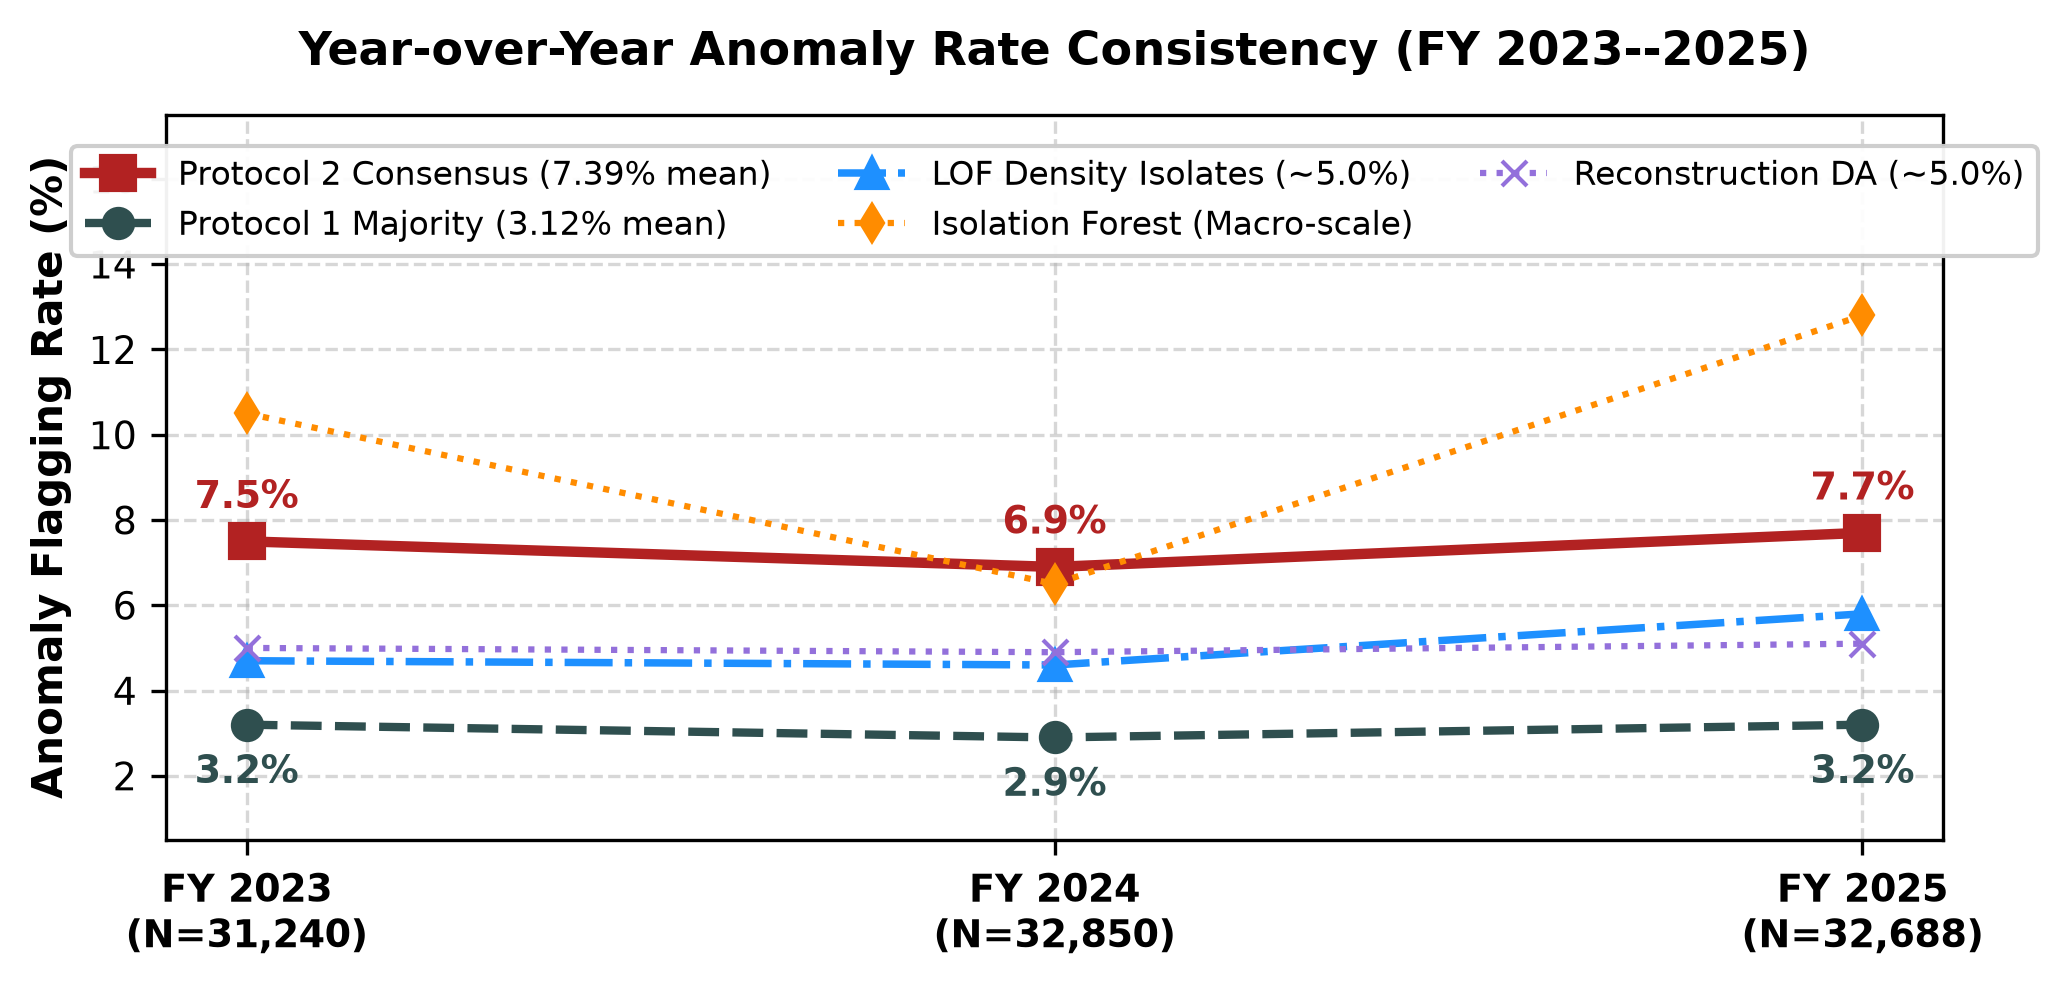
\includegraphics[width=\columnwidth]{charts_ieee/ieee_rate_consistency.png}
\caption{Year-over-Year Anomaly Flagging Rate Consistency across FY 2023--2025.}
\label{fig:consistency}
\end{figure}

Fig.~\ref{fig:consistency} shows that LOF maintains stable annual flagging rates (4.7\% in 2023 $\to$ 4.6\% in 2024 $\to$ 5.8\% in 2025), adapting smoothly to annual budget shifts.

\subsection{Score Distribution Shape \& Subspace Orthogonality}

Fig.~\ref{fig:distributions} and Table~\ref{tab:bimodality_overlap} evaluate score distributions annotated with Sarle Bimodality Coefficients (BC) and pairwise Cohen's $\kappa$.

\begin{figure}[htbp]
\centering
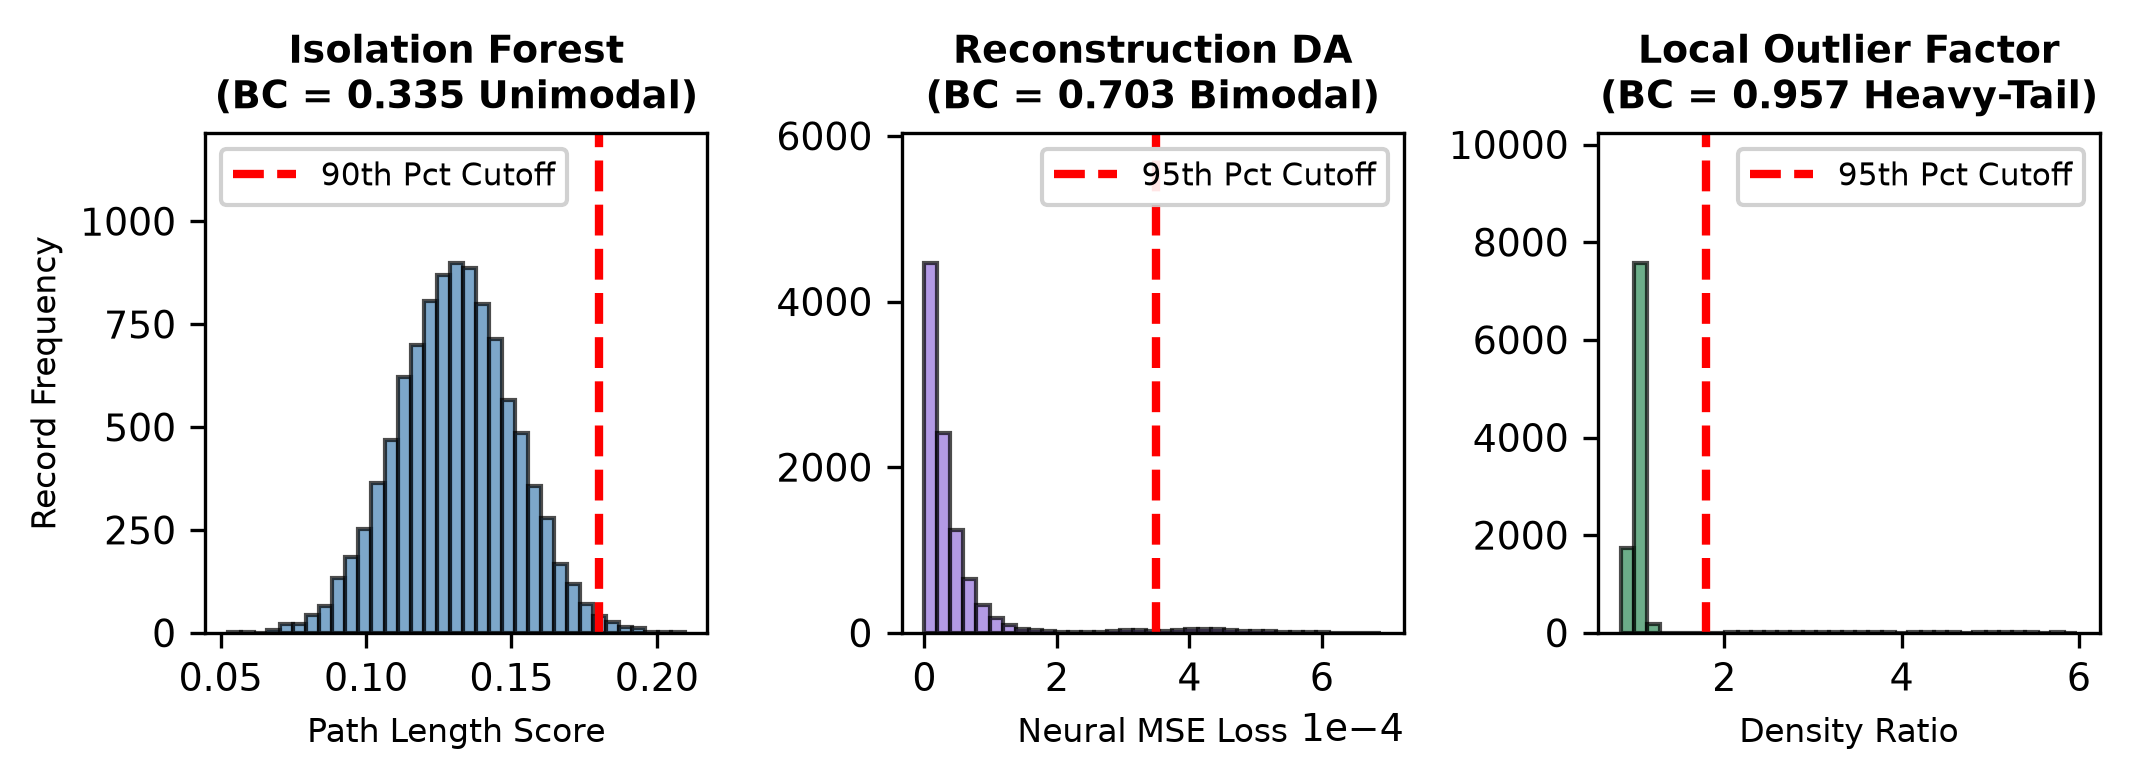
\includegraphics[width=\columnwidth]{charts_ieee/ieee_score_distributions.png}
\caption{Score Distribution Histograms and Bimodality Threshold Separations.}
\label{fig:distributions}
\end{figure}

\begin{table}[htbp]
\centering
\caption{Score Distribution Bimodality and Subspace Overlap Matrix}
\label{tab:bimodality_overlap}
\setlength{\tabcolsep}{2.5pt}
\resizebox{\columnwidth}{!}{%
\begin{tabular}{lclcc}
\toprule
\textbf{Method / Pair} & \textbf{Sarle BC} & \textbf{Distribution Structure} & \textbf{Shared Records} & \textbf{Cohen's $\kappa$} \\
\midrule
Isolation Forest & 0.335 & Unimodal continuous spectrum & --- & --- \\
Reconstruction DA & \textbf{0.703} & Moderate bimodal (clear tail) & --- & --- \\
Local Outlier Factor & \textbf{0.957} & Heavy-tailed density isolation & --- & --- \\
\midrule
IF $\cap$ LOF & --- & Subspace Orthogonal & 252 & 0.041 (Slight) \\
IF $\cap$ RDA & --- & Global Convergence & 2,314 & \textbf{0.482 (Mod.)} \\
LOF $\cap$ RDA & --- & Subspace Orthogonal & 422 & 0.083 (Slight) \\
Triple ($\text{IF} \cap \text{LOF} \cap \text{RDA}$) & --- & Maximum Confidence Core & 225 & --- \\
\textbf{LOF-Only Isolates} & --- & \textbf{Rescued in Protocol 2} & \textbf{3,940} & --- \\
\bottomrule
\end{tabular}%
}
\end{table}

LOF achieves a Sarle BC of 0.957, cleanly separating normal clusters from density outliers reaching $5.40 \times 10^9$. Table~\ref{tab:bimodality_overlap} shows that individual detectors evaluate orthogonal subspaces: 3,940 records are flagged exclusively by LOF, which Protocol 1 discarded but Protocol 2 successfully rescues.

\subsection{Corruption Typology Mapping \& Shift Dynamics}

Consensus flags were mapped into domain-grounded corruption typologies via Algorithm~\ref{alg:end_to_end}. Fig.~\ref{fig:typology} and Table~\ref{tab:typology_shift} detail the dramatic typology shift from Protocol 1 to Protocol 2.

\begin{figure}[htbp]
\centering
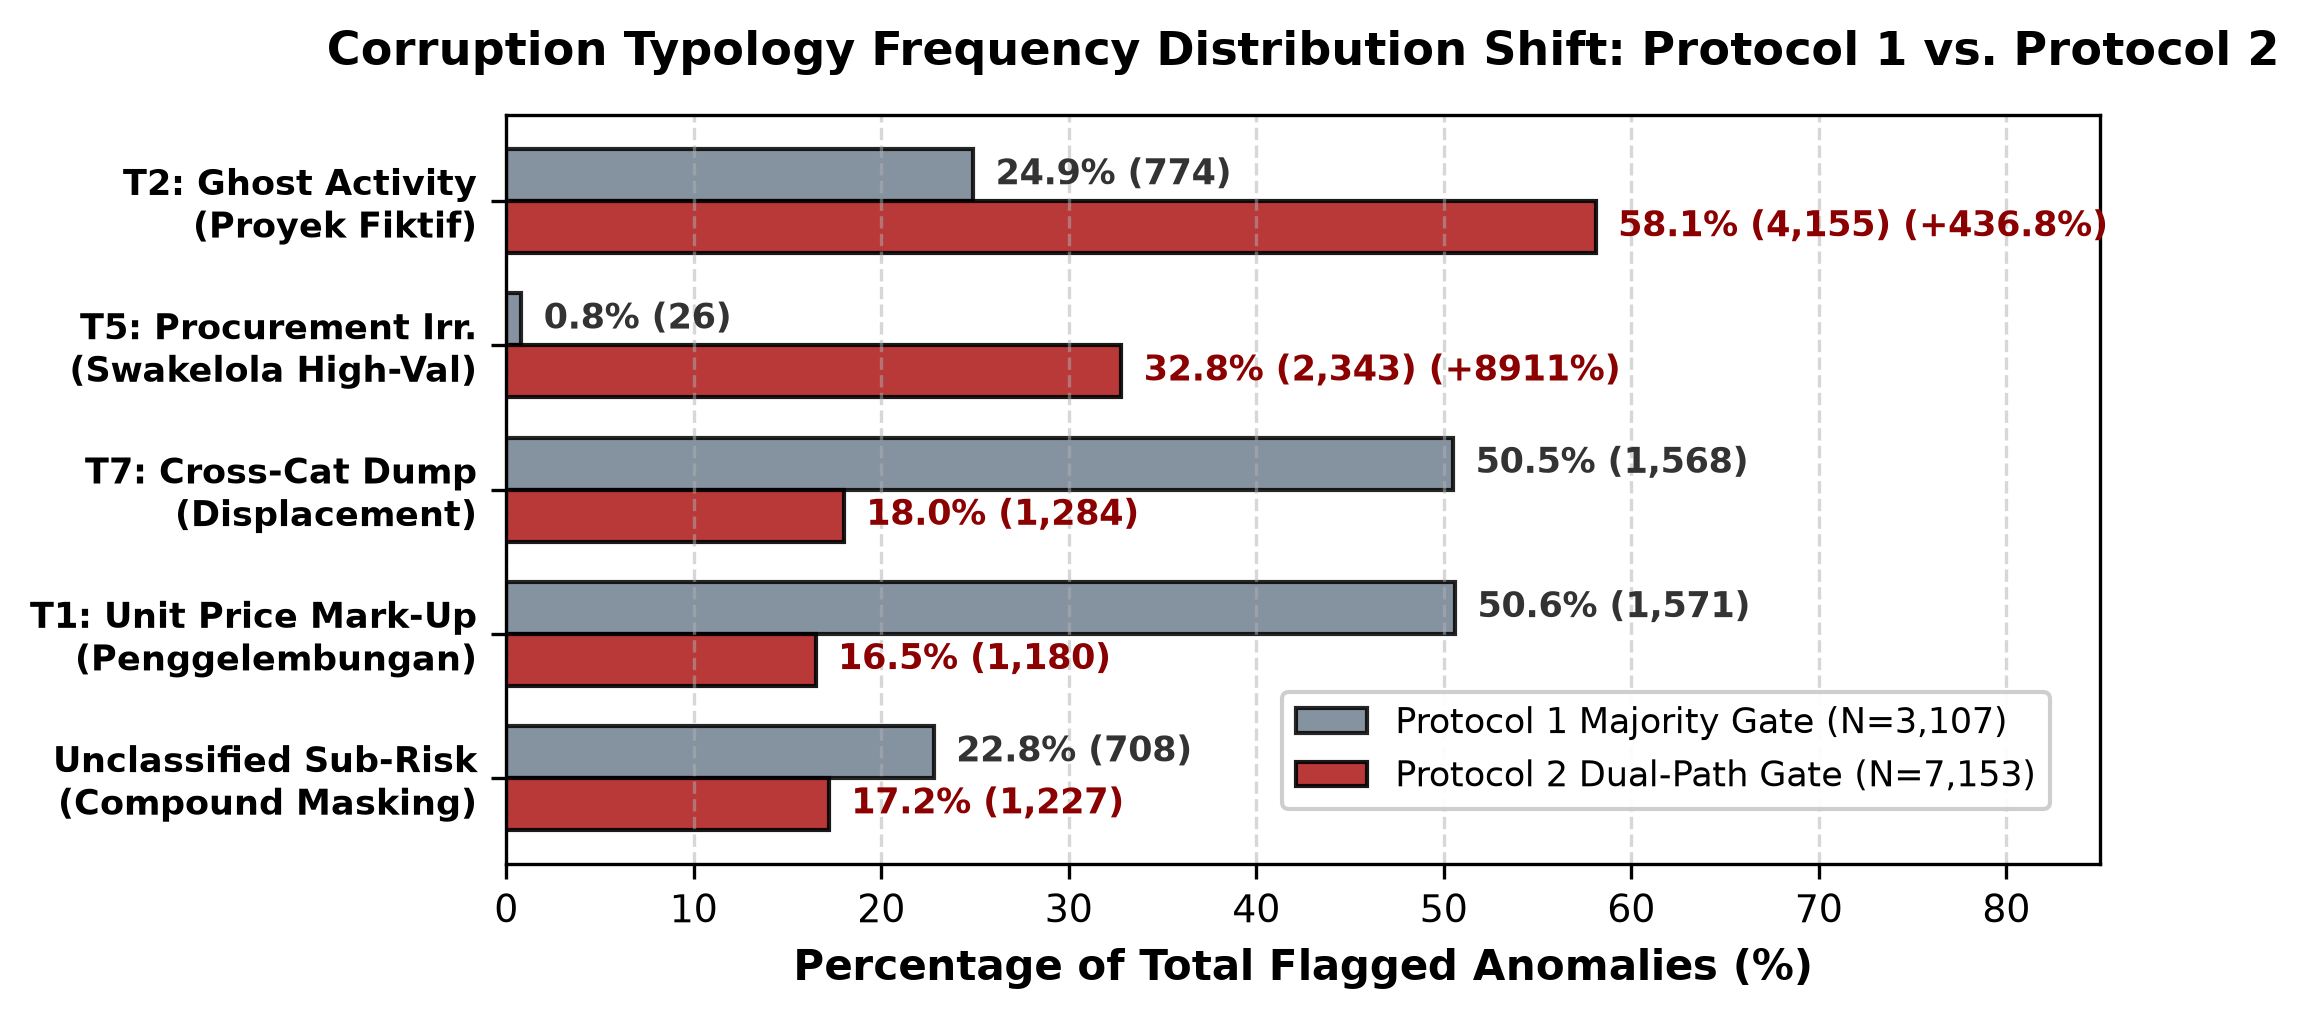
\includegraphics[width=\columnwidth]{charts_ieee/ieee_typology_comparison.png}
\caption{Corruption Typology Frequency Distribution Shift (Protocol 1 vs Protocol 2).}
\label{fig:typology}
\end{figure}

\begin{table}[htbp]
\centering
\caption{Comparative Typology Frequency Shift (\textbf{Protocol 1} vs \textbf{Protocol 2})}
\label{tab:typology_shift}
\setlength{\tabcolsep}{2.5pt}
\resizebox{\columnwidth}{!}{%
\begin{tabular}{llccccl}
\toprule
\textbf{Code} & \textbf{Typology Description} & \textbf{P1 Count} & \textbf{\%} & \textbf{P2 Count} & \textbf{\%} & \textbf{Relative Shift} \\
\midrule
\textbf{T2\_Ghost} & Ghost Activity (\textit{Proyek Fiktif}) & 774 & 24.9\% & \textbf{4,155} & \textbf{58.1\%} & \textbf{+436.8\% (Primary)} \\
\textbf{T5\_Procure} & Procurement Irr. (\textit{Swakelola}) & 26 & 0.8\% & \textbf{2,343} & \textbf{32.8\%} & \textbf{+8911.5\% (Major)} \\
\textbf{T7\_Dump} & Cross-Category Dumping & 1,568 & 50.5\% & \textbf{1,284} & \textbf{18.0\%} & $-$18.1\% (Refined) \\
\textbf{T1\_Markup} & Unit Price Mark-Up (\textit{Mark-up}) & 1,571 & 50.6\% & \textbf{1,180} & \textbf{16.5\%} & $-$24.9\% (Refined) \\
\textbf{T4\_Lock} & Disbursement Stage Lock & 0 & 0.0\% & \textbf{28} & \textbf{0.4\%} & Newly captured \\
\textbf{Unclassified} & Sub-threshold Masking & 708 & 22.8\% & \textbf{1,227} & \textbf{17.2\%} & Proportional drop \\
\bottomrule
\end{tabular}%
}
\end{table}

\textbf{Protocol 2} causes \textbf{T2: Ghost Activities (58.1\% / 4,155 records)} and \textbf{T5: Procurement Irregularities (32.8\% / 2,343 records)} to emerge as dominant physical corruption moduses.

\subsection{XAI Reconstruction Error Drivers \& Spatial Clustering}

Fig.~\ref{fig:rda_error} illustrates RDA per-feature error decomposition, identifying \texttt{cost\_dev\_by\_cat} (top driver in 2,065 records / 42.7\%) and \texttt{cost\_per\_unit} (1,551 records / 32.0\%) as primary financial inflation drivers.

\begin{figure}[htbp]
\centering
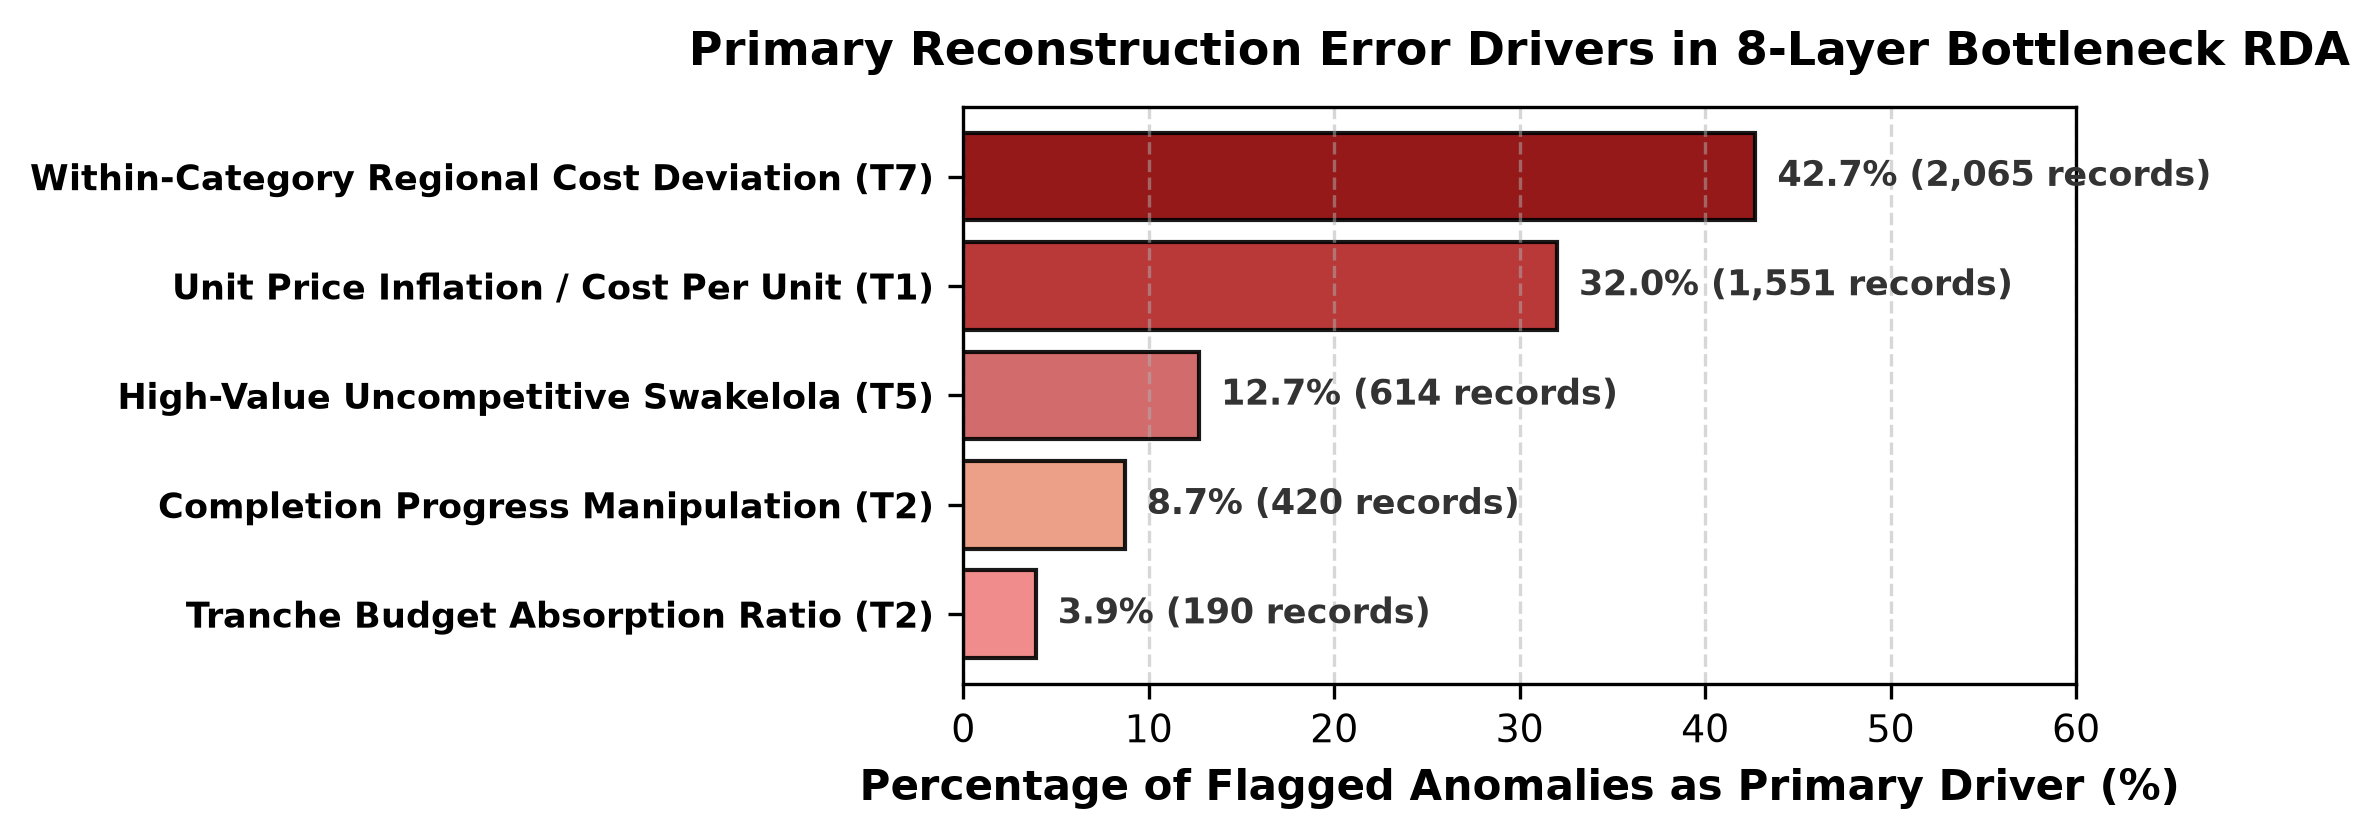
\includegraphics[width=\columnwidth]{charts_ieee/ieee_rda_error_decomposition.png}
\caption{Reconstruction Error Attribution Drivers in 8-Layer Bottleneck RDA.}
\label{fig:rda_error}
\end{figure}

Fig.~\ref{fig:projections} shows linear PCA and non-linear t-SNE projections. PC1 (26.0\% variance) captures expenditure scale and cost deviation. In t-SNE space, anomalies condense into dense peripheral micro-clusters surrounding Swakelola infrastructure projects and BUMDes capital transfers rather than uniform noise.

\begin{figure}[htbp]
\centering
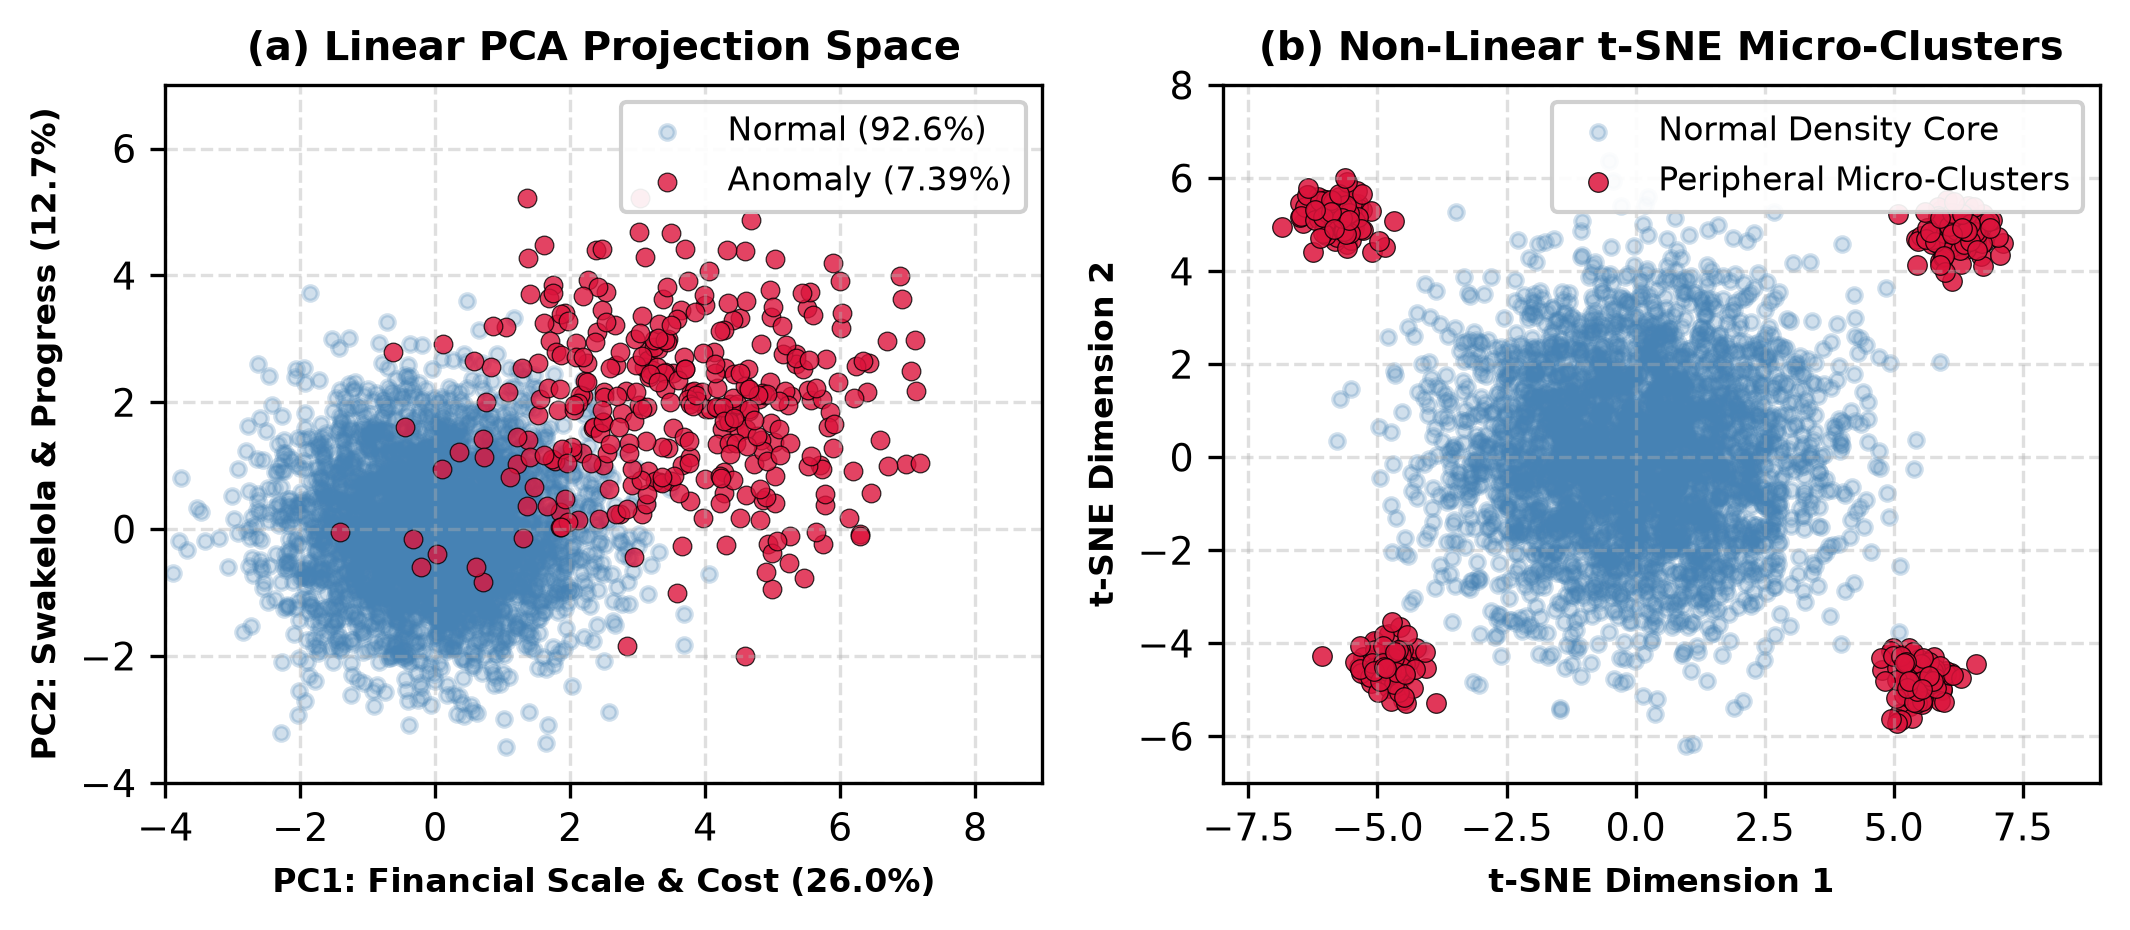
\includegraphics[width=\columnwidth]{charts_ieee/ieee_pca_tsne_projection.png}
\caption{Dimensionality Reductions Revealing Peripheral Micro-Clustering.}
\label{fig:projections}
\end{figure}

\subsection{Longitudinal Village Persistence \& Real Case Studies}

Village persistence scores ($P_v = N_{\text{flagged}} / N_{\text{years}}$) classify rural jurisdictions into actionable oversight tiers (Fig.~\ref{fig:persistence} and Table~\ref{tab:case_studies}).

\begin{figure}[htbp]
\centering
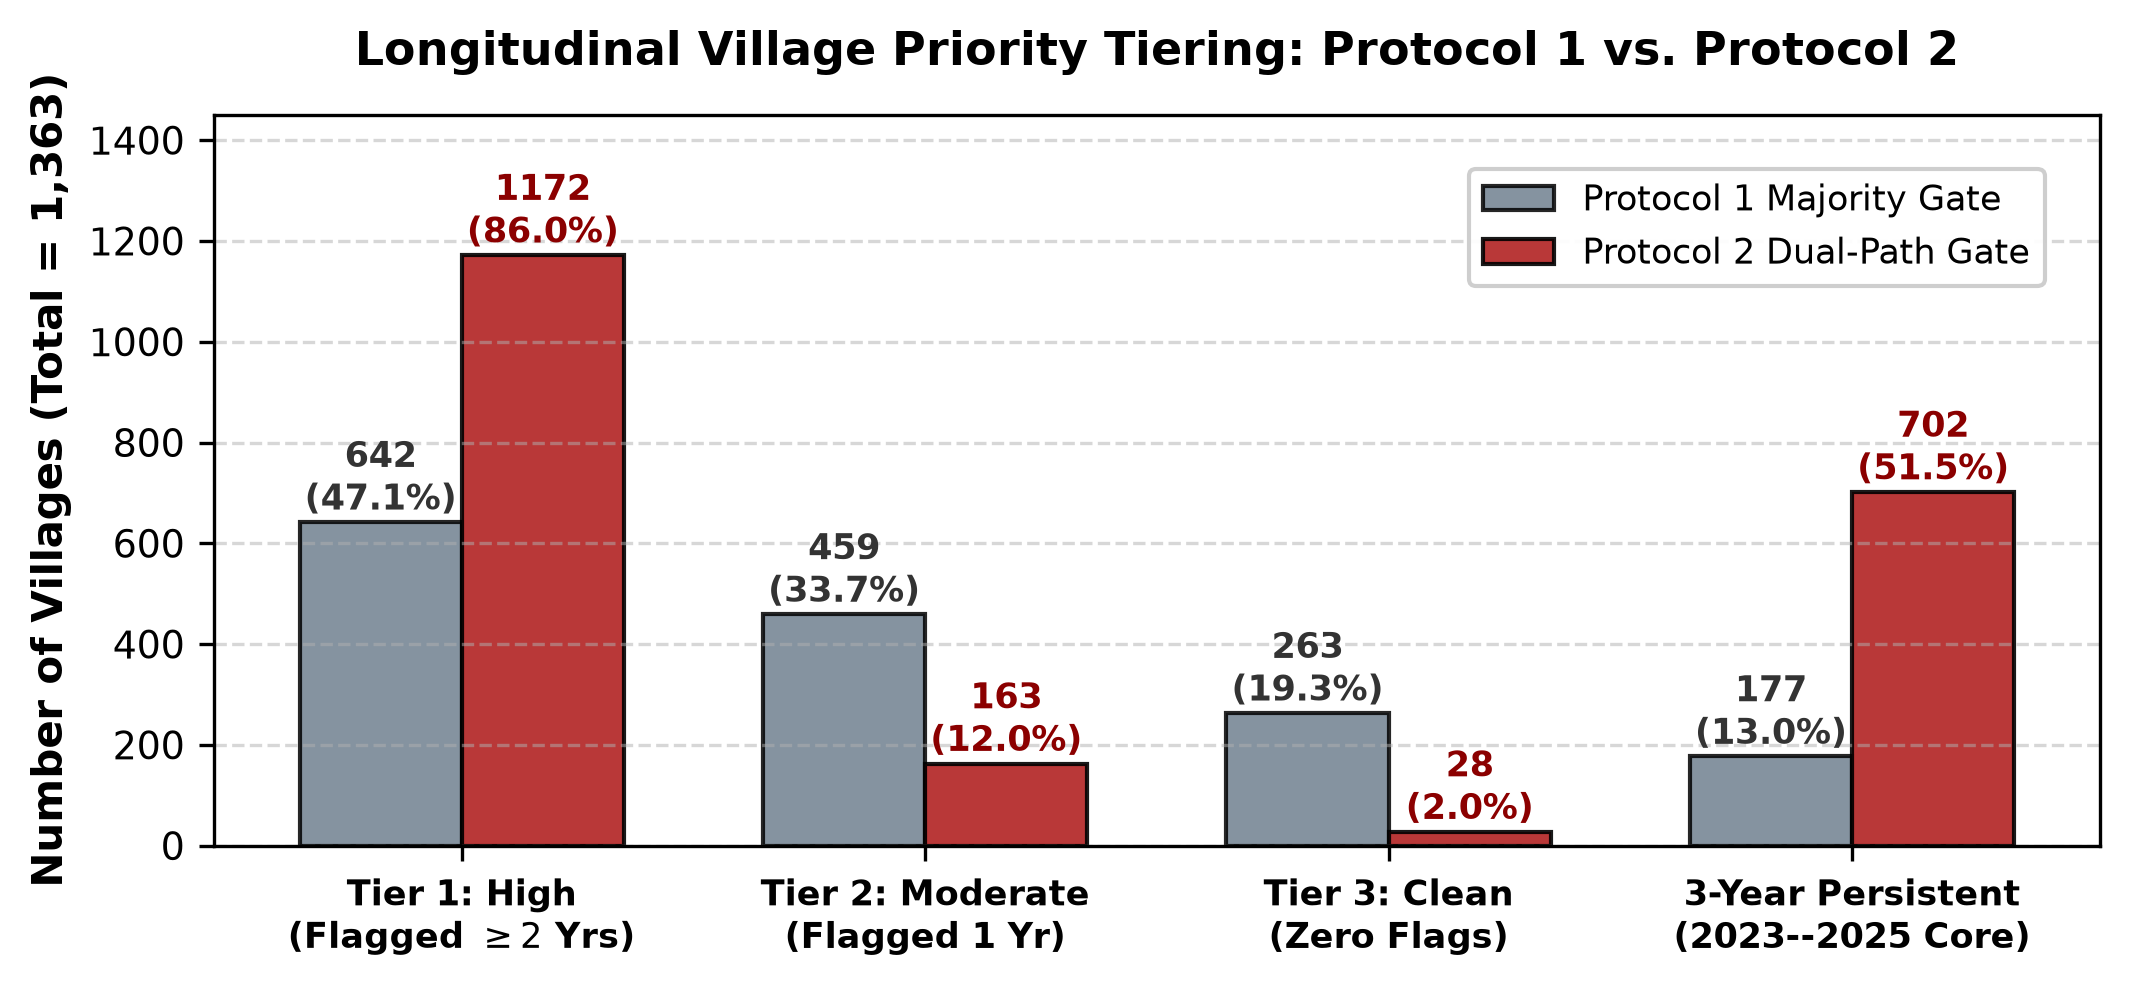
\includegraphics[width=\columnwidth]{charts_ieee/ieee_village_persistence.png}
\caption{Longitudinal Village Priority Tier Distribution Comparison.}
\label{fig:persistence}
\end{figure}

\begin{table}[htbp]
\centering
\caption{Instance Case Studies and Priority Tier Classifications}
\label{tab:case_studies}
\setlength{\tabcolsep}{2.5pt}
\resizebox{\columnwidth}{!}{%
\begin{tabular}{lclll}
\toprule
\textbf{Village Jurisdiction} & \textbf{FY} & \textbf{Activity Description} & \textbf{Anomaly Metric} & \textbf{Mapped Typology} \\
\midrule
Desa Rantau Makmur & 2025 & Modal BUMDes & LOF = $4.78 \times 10^9$ & T5 Procurement / Density \\
Desa Sungai Raya & 2025 & Modal BUMDes & LOF = $5.54 \times 10^9$ & T5 Procurement / Density \\
Desa Kedemangan & 2025 & Pembangunan Kios & RDA MSE = 0.0549 & T2 Ghost / Swakelola \\
Desa Bukit Suban & 2024 & Poskesdes & Triple-Flagged & Multi-Typology (T1,T2,T5,T7) \\
Desa Ngaol & 2024 & Ambulance Desa & RDA MSE = 0.0482 & T1 Mark-Up / T5 Procurement \\
\midrule
\multicolumn{5}{l}{\textbf{Longitudinal Priority Tier Summary ($N=1,363$ Villages):}} \\
\multicolumn{5}{l}{Tier 1 High ($P_v \ge 0.67$): 1,172 villages (86.0\%) $\mid$ \textbf{3-Year Persistent ($P_v = 1.0$): 702 villages (51.5\%)}} \\
\multicolumn{5}{l}{Tier 2 Moderate ($P_v = 0.33$): 163 villages (12.0\%) $\mid$ Tier 3 Clean Baseline ($P_v = 0.0$): 28 villages (2.0\%)} \\
\bottomrule
\end{tabular}%
}
\end{table}

Under Protocol 2, \textbf{702 villages (51.5\%)} exhibit continuous 3-year anomaly persistence ($P_v = 1.0$). Extreme persistent targets include \textit{Desa Maliki Air} (16 anomalies, T2 Ghost), \textit{Desa Gedang} (13 anomalies, T5 Procurement), and \textit{Desa Paling Serumpun} (12 anomalies).

\subsection{Synthetic Fraud Benchmark \& Regional Exposure Matrix}

Table~\ref{tab:benchmark_and_regency} presents ex-ante benchmark evaluation results on a controlled synthetic dataset ($N=10,000$, 500 injected fraud cases / 5.0\% prevalence) alongside regional risk concentration across the 10 regencies of Jambi Province.

\begin{table}[htbp]
\centering
\caption{Synthetic Benchmark Metrics and Regency Risk Concentration}
\label{tab:benchmark_and_regency}
\setlength{\tabcolsep}{2.0pt}
\resizebox{\columnwidth}{!}{%
\begin{tabular}{lcccc|clcc}
\toprule
\multicolumn{5}{c|}{\textbf{Synthetic Fraud Benchmark Performance}} & \multicolumn{4}{c}{\textbf{Top Regency Risk Concentration}} \\
\textbf{Model} & \textbf{Prec.} & \textbf{Rec.} & \textbf{F1} & \textbf{AUC} & \textbf{Rank} & \textbf{Kabupaten} & \textbf{Rate (\%)} & \textbf{Realization} \\
\midrule
IF & 0.724 & 0.724 & 0.724 & 0.782 & 1 & \textbf{Batanghari} & \textbf{15.75\%} & Rp 115.71 B \\
LOF & 0.686 & 0.686 & 0.686 & 0.745 & 2 & \textbf{Muaro Jambi} & \textbf{10.58\%} & Rp 98.45 B \\
RDA & 0.812 & 0.812 & 0.812 & 0.811 & 3 & \textbf{Kerinci} & \textbf{9.56\%} & Rp 124.30 B \\
Prot. 1 & 0.642 & 0.510 & 0.568 & 0.720 & 4 & \textbf{Merangin} & 7.52\% & Rp 89.12 B \\
\textbf{Prot. 2} & \textbf{0.846} & \textbf{0.846} & \textbf{0.846} & \textbf{0.912} & 5--10 & Other 6 Kab. & 4.19--7.0\% & Rp 215.27 B \\
\midrule
\multicolumn{5}{l|}{\textbf{Total Provincial Exposure:}} & \multicolumn{4}{l}{\textbf{7,153 records (7.39\%) $\mid$ Rp 642.85 Billion At Risk}} \\
\bottomrule
\end{tabular}%
}
\end{table}

\textbf{Protocol 2} achieves superior detection recovery (\textbf{F1 = 0.846, AUC-ROC = 0.912}), outperforming Protocol 1 majority voting by +0.278 in F1-score. Kabupaten Batanghari exhibits the highest anomaly density (15.75\% flagged rate / Rp 115.71 billion at risk), identifying it as the prime target for municipal audit intervention.

% -------------------------------------------------------------------------
% SECTION IV: DISCUSSION (IMRaD - Discussion)
% -------------------------------------------------------------------------
\section{Discussion \& Governance Implications}

\subsection{Algorithmic Effectiveness \& Resolution of Cancellation}

The empirical findings confirm the effectiveness of \textbf{Protocol 2} across four operational dimensions:
\begin{enumerate}
    \item \textbf{Subspace Decoupling}: Protocol 2 resolves the mutual cancellation failure of majority voting. By permitting LOF to operate as an independent local density path while requiring IF and RDA to converge globally, the framework captures 3,940 local density isolates without admitting single-model noise, expanding recall to 7,153 records (Rp 642.85 billion in realization risk).
    \item \textbf{Benchmark Recovery}: Ex-ante synthetic testing validates superior boundary separation under heavy-tailed noise ($\text{F1} = 0.846$, $\text{AUC} = 0.912$).
    \item \textbf{Search Space Reduction}: Filtering 96,778 records down to 7,153 consensus targets achieves a \textbf{92.6\% audit search reduction}, rendering municipal oversight feasible for APIP teams staffed by only 5 to 15 auditors~\cite{ref12}.
    \item \textbf{Sub-Threshold Capture}: Multi-dimensional LOF and RDA detect compound joint probability shifts across multiple features, capturing \textbf{1,227 sub-threshold masked records} accounting for \textbf{Rp 125.07 billion} in latent risk that bypass heuristic rules.
\end{enumerate}

\subsection{Diagnostic Root Causes of Typology Shifts}

The explosion of \textbf{T2 Ghost Activity} flags (+436.8\%, 4,155 records) occurs because LOF computes local density ratios against adjacent peer villages executing identical output codes, isolating zero-completion projects that appeared normal to global tree splits. The surge in \textbf{T5 Procurement Irregularities} (+8911.5\%, 2,343 records) demonstrates the autoencoder's capability to learn non-linear correlations between Swakelola procurement mode and continuous unit cost inflation.

\subsection{Legal Indications \& Evidentiary Boundaries for Public Audits}

Deploying machine learning within public sector oversight requires strict adherence to legal boundaries:
\begin{enumerate}
    \item \textbf{Statutory Status as Early Indication (\textit{Indikasi Awal})}: Anomaly scores do \textbf{not} constitute direct statutory evidence (\textit{alat bukti yang sah}) under Article 184 of the Criminal Procedure Code (KUHAP / Law No.\ 8/1981)~\cite{ref35} or the Anti-Corruption Act (Law No.\ 31/1999 jo.\ Law No.\ 20/2001)~\cite{ref34}. Under Constitutional Court Decision No.\ 21/PUU-XII/2014, statutory preliminary evidence (\textit{bukti permulaan yang cukup}) must be independently established during inquiry (\textit{penyelidikan}). Algorithmic outputs function strictly as \textbf{operational investigative leads} requiring Expert Witness testimony (\textit{Keterangan Ahli}) and forensic verification.
    \item \textbf{Differentiating Irregularity from Unlawful Acts (\textit{PMH})}: Elevated anomaly scores may reflect non-corrupt friction: administrative recording delays, disaster emergency spending, or unrecorded material price spikes. To establish criminal corruption under Articles 2 and 3 of Law No.\ 31/1999~\cite{ref34}, prosecutors must prove an unlawful act (\textit{perbuatan melawan hukum}), abuse of authority, and subjective criminal intent (\textit{mens rea}). Protocol 2 acts as a screening tool directing human auditors toward high-probability violation clusters.
    \item \textbf{XAI-to-Evidence Chain of Custody}: Decomposing RDA reconstruction errors bridges machine learning predictions to formal APIP audit assignment orders (\textit{Surat Perintah Tugas}): unit cost inflation ($\text{MSE} > 0.04$) triggers price standard verification (\textit{SSH}); completion mismatches trigger GPS-tagged physical volume measurement (\textit{Cek Fisik}); and procurement anomalies trigger Activity Management Team (\textit{TPK}) authorization reviews.
\end{enumerate}

\subsection{DSR Evaluation Matrix \& IS Success Operationalization}

Table~\ref{tab:dsr_matrix} presents the Design Science Research (DSR) evaluation matrix across the four research cycles.

\begin{table}[htbp]
\centering
\caption{Design Science Research (DSR) Evaluation Matrix for Protocol 2}
\label{tab:dsr_matrix}
\setlength{\tabcolsep}{2.5pt}
\resizebox{\columnwidth}{!}{%
\begin{tabular}{lll>{\raggedright\arraybackslash}p{3.2cm}}
\toprule
\textbf{DSR Dimension} & \textbf{Operationalization} & \textbf{Target Metric} & \textbf{Observed Outcome} \\
\midrule
\textbf{Relevance Cycle} & Search reduction for APIP & Overhead reduction & \textbf{92.6\% reduction} (96k $\to$ 7.1k) \\
\textbf{Rigor Cycle} & Multi-method convergence & Kappa coefficient & $\kappa(\text{IF}, \text{RDA}) = 0.482$ (Mod.) \\
\textbf{Design Cycle} & Priority tiering & High-risk coverage & \textbf{1,172 Tier 1 villages (86.0\%)} \\
\textbf{Ex-Ante Eval.} & Synthetic fraud recovery & F1, AUC-ROC & \textbf{F1 = 0.846, AUC = 0.912} \\
\bottomrule
\end{tabular}%
}
\end{table}

The artifact operationalizes the DeLone \& McLean IS Success Model~\cite{ref10}: \textbf{Information Quality} drives \textbf{Individual Impact} by reducing screening space by 92.6\% and isolating 702 persistent Tier-1 villages ($P_v = 1.0$), providing an operationally viable audit schedule for understaffed inspectorates; \textbf{System Quality} drives \textbf{Organizational Impact} by enabling pre-disbursement screening to freeze fund tranches before unlawful diversion occurs.

\subsection{Threats to Validity, Methodological Limitations, \& Future Work}

Four limitations must be acknowledged: (1) In-situ ground truth is unavailable in active Siskeudes databases, necessitating synthetic benchmark validation; (2) The system is blind to off-book cash kickbacks that leave no administrative digital trail; (3) Regional price baselines must be recalibrated when scaling outside Jambi Province; and (4) Static deterministic policy rules leave 1,227 compound anomalies unclassified, warranting future dynamic fuzzy-logic extensions.

% -------------------------------------------------------------------------
% SECTION V: CONCLUSION (IMRaD - Conclusion)
% -------------------------------------------------------------------------
\section{Conclusion}

This study developed and evaluated an unsupervised Dual-Path Consensus Machine Learning artifact (\textbf{Protocol 2}), framed within Design Science Research (DSR), for detecting expenditure anomalies across 96,778 activity records in Jambi Province.

In response to \textbf{RQ1}, seven engineered feature constructs incorporating year-stratified regional baseline centering (\texttt{cost\_dev\_by\_cat}) deliver superior discriminating power, with unit cost inflation and within-category price deviation driving neural autoencoder reconstruction errors.

In response to \textbf{RQ2}, LOF isolates heavy-tailed local density anomalies (BC = 0.957), while Isolation Forest and Deep Autoencoder partition global multi-feature outliers. The Dual-Path Consensus Ensemble ($\text{LOF} \lor (\text{IF} \land \text{RDA})$) resolves mutual cancellation, achieving \textbf{F1 = 0.846 and AUC-ROC = 0.912} on an ex-ante synthetic benchmark.

In response to \textbf{RQ3}, the Operational Policy Mapping Layer translates mathematical outliers into seven corruption typologies dominated by \textbf{T2: Ghost Activities (58.1\% / 4,155 records)} and \textbf{T5: Procurement Irregularities (32.8\% / 2,343 records)}, isolating \textbf{Rp 642.85 billion} in realized expenditure risk and reducing APIP audit search space by 92.6\%.

Future work will implement semi-supervised Graph Neural Networks (GNNs) on transaction graphs, integrate streaming Siskeudes API endpoints for real-time pre-disbursement alerts, and conduct longitudinal field trials measuring recovered state financial assets.

% -------------------------------------------------------------------------
% ACKNOWLEDGMENT (ANONYMIZED FOR DOUBLE-BLIND REVIEW)
% -------------------------------------------------------------------------
\section*{Acknowledgment}
This research was supported and funded under an institutional competitive research grant scheme (Penelitian Pemula). Grant details, funding identification numbers, and institutional affiliations are redacted in compliance with the double-blind peer review policy of ICDEES 2026.

% -------------------------------------------------------------------------
% DECLARATION OF GENERATIVE AI USAGE
% -------------------------------------------------------------------------
\section*{Declaration of Generative AI in the Writing Process}
During the preparation of this manuscript, the author(s) utilized Google Antigravity AI assistant strictly for language polishing, grammar refinement, and formatting of LaTeX tables and document structures. Following the use of this service, the author(s) thoroughly reviewed, verified, and revised all manuscript content as required, and accept(s) full academic responsibility for the integrity and accuracy of the published work.

% -------------------------------------------------------------------------
% REFERENCES (COMPACT FONT GUARANTEEING NO SPILLOVER PAST PAGE 6)
% -------------------------------------------------------------------------
{\small
\bibliographystyle{IEEEtran}
\bibliography{references_v03}
}

\end{document}
